% 02.06.2016 12:00 CET last changed by a.holzinger
% General Template for LNCS and LNAI contributions based on llncs, adapted by ah
% Many thanks to the TRS team
% In case of using eps compile via 1) TeXify and then proceed with 2) dvi2pdf
%
\documentclass{llncs}
\usepackage{float}

\usepackage[dvips]{graphicx}
\usepackage[ruled,vlined]{algorithm2e}
\usepackage{amsfonts}
\usepackage{amssymb}
\usepackage{amsmath}
\usepackage{mathtools}

\providecommand{\abs}[1]{\lvert#1\rvert}
\providecommand{\norm}[1]{\lVert#1\rVert}

\usepackage{calc}
\usepackage{subfigure}

\usepackage{color}
\usepackage{soul}
\usepackage{comment}

\newtheorem{prop}{Property}

\newenvironment{Bitemize}{\renewcommand\labelitemi{\textbullet}\begin{itemize}}{\end{itemize}}

\begin{document}

\title{Interactive Anonymization\\
for Privacy aware Machine Learning}

\author{Bernd Malle\inst{1}\inst{2}, Peter Kieseberg\inst{1}\inst{2}, Andreas Holzinger\inst{1}}

\institute{Holzinger Group HCI-KDD \\
Institute for Medical Informatics, Statistics \& Documentation\\
            Medical University Graz, Austria\\
            \texttt{b.malle@hci-kdd.org}
\and
SBA Research gGmbH, Favoritenstraße 16, 1040 Wien \\
			\texttt{PKieseberg@sba-research.org}
}
	
\maketitle

% ==================================
%				ABSTRACT
% ==================================
\begin{abstract}

Privacy aware Machine Learning is the discipline of applying Machine Learning techniques in such a way as to protect personal identities during the process. This can most easily be achieved by first anonymizing a dataset before releasing it for the purpose of statistical data mining or research; starting in June 2018, this will also remain the sole legally permitted way within the European Union to release data without granting persons involved the 'right to be forgotten', i.e. the right to have their data deleted on request. To governments, organizations and corporations however, this represents a serious impediment to research operations, since any anonymization results in a certain degree of information loss and therefore reduced data utility. Our work focuses on applying interactive Machine Learning to the process of anonymization based on the idea of eliciting human background knowledge to optimize an algorithm's parameters as to which attributes are more or less valuable for preservation. Our experiments show that human knowledge can yield measurably better classification results than a rigid automatic approach, whereas the impact of interactive learning in the field of anonymization will largely depend on the experimental setup as well as suitable choices of application domains as well as human test subjects.


\medskip

\textbf{Keywords}: Machine Learning, Privacy aware ML, interactive ML, Knowledge Bases, Anonymization, k-Anonymity, SaNGreeA, Information Loss, Weight Vectors


\end{abstract}

\renewcommand{\thesubfigure}{\thefigure.\arabic{subfigure}}
\makeatletter
\renewcommand{\p@subfigure}{}
\renewcommand{\@thesubfigure}{\thesubfigure:\hskip\subfiglabelskip}
\makeatother


% ==================================
%			INTRODCUTION
% ==================================
\section{Introduction and Motivation}
\label{sect:intro_moti}



This original requirement of \textit{k-anonymity} \cite{Sweeney:2002:k-Anonymity} has since been extended by the concepts of \textit{l-diversity} \cite{MachanavajjhalaEtAl:2007:l-Diversity} (where every cluster must contain at least $l$ diverse sensitive values), \textit{t-closeness} \cite{LiEtAl:2007:t-closeness} (demanding that the local distribution over sensitive values must not diverge from its global distribution by more than a factor of $t$) as well as \textit{delta-presence} \cite{NergizClifton:2010:Delta-Presence} (which incorporates the background knowledge of a potential attacker). Although all of those concepts are interesting in their own right, for the sake of comparing interactive ML algorithms to  their fully automatic counterpart, we only took \textit{k-anonymity} into consideration (at least for this work).

based on our initial PAML experiments \cite{}



% ==================================
%			  K-ANON
% ==================================
\section{k-anonymity (and beyond)}
\label{sect:k_anon}

Given the original tabular concept of anonymization, we will usually encounter three different categories of attributes within a given dataset:

\begin{itemize}
	\item \textbf{Personal identifiers} are data items which directly identify a person without having to cross-reference or further analyze them. Examples are email address or social security number (SSN). As personal identifiers are immediately dangerous, this category of data is usually removed.
	\item \textbf{Sensitive data,} also called 'payload', represents information that is crucial for further data mining or research purposes. Examples for this category would be disease classification, drug intake or personal income. This data shall be preserved in the anonymized dataset and can therefore not be deleted or generalized.
	\item \textbf{Quasi identifiers (QI's)}, are data which in themselves do not directly reveal the identity of a person, but might be used in aggregate to reconstruct it. For instance, \cite{sweeney2002k} reported in 2002 that the identity of 87\% of U.S. citizens could be uncovered via just the 3 attributes \textit{zip code}, \textit{gender} and \textit{date of birth}. Despite this danger, QI's may contain vital information to research applications (like ZIP code in a disease spread study); they are therefore generalized to an acceptable compromise between privacy (data loss) and information content (data utility).
\end{itemize}

Based on this categorization \textit{k-anonymity} \cite{Samarati:2001:kAnonymity} was introduced as a formal concept of privacy , in which a record is released only if its quasi-identifiers are indistinguishable from at least $k-1$ other entities in the dataset. This can be imagined like a clustering of data into so-called \textit{equivalence classes} of at least size $k$, with all internal QI's being generalized to the exact same level.

Generalization in this setting means an abstraction of attribute value: e.g. given two ZIP codes of '8010' and '8045', we could first generalize to '80**', then incorporate another data point showing ZIP '8500' by generalizing the cluster to '8***', and finally merging with any other ZIP code to the highest level of 'all', also denoted as '*'.


% ==================================
%				iML
% ==================================
\section{interactive Machine Learning}
\label{sect:iML}

Interactive ML algorithms adjust their inner workings by continuously interacting with an outside \textit{oracle}, drawing positive / negative reinforcement from this interaction \cite{Holzinger:2016:iML}. Such systems are especially useful for highly-personalized predictions or decision support \cite{Kieseberg:2016:Doctor-in-the-Loop}; moreover many real-world problems exhibit (super)exponential algorithmic runtime; in such cases human brains dwarf machines at approximating solutions and learning from very small samples, thus enabling us to 'intuit' solutions efficiently \cite{iMLExperiment}.

By incorporating humans as oracles into this process, we can elicit background knowledge regarding specific use cases unknown to automatic algorithms \cite{WARE2001}. This however is highly dependent on the users' experience in a certain field as well as data / classification complexity; domain experts can of course be expected to contribute more valuable decision points than laymen; likewise, a low-dimensional dataset and simple classification tasks will result in higher quality human responses than convoluted problem sets.

While the authors of \cite{Moque2012} propose a system that interacts with a user in order to set a certain k-factor and subsequently provides a report on information loss and Kurtosis of QI distributions, the algorithm is not \textit{interactive} by our definition in that it does not influence the inner workings of the algorithm during the learning phase. This is also true in case of the Cornell Anonymization Toolkit (Cat) \cite{Xiao2009}, which conducts a complete anonymization run and only then lets the user decide if they are content with the results. In contrast, our approach alters algorithmic parameters upon every (batch of) human decisions, letting the algorithm adapt in real-time.

\cite{Loh2010} describe an approach incorporating humans into the anonymization process by allowing them to set constraints on attribute generalization; moreover they construct generalization hierarchies involving domain-specific ontologies. Although this technique marks a departure from wholesale automatic anonymization, it still lacks the dynamic human-computer interaction of our approach.

Apart from the field of privacy, interactive ML is today present in a wide spectrum of applications, from bordering medical fields like protein interactions / clusterings \cite{Amershi2014} via on-demand group-creation in social networks \cite{Amershi2012} to even teaching algorithms suitable mappings from gestures to music-generating parameters \cite{Fiebrink2009}.



% ==================================
%			EXPERIMENTS
% ==================================
\section{Experiments}
\label{sect:experiments}

The following sections will describe our experiment in detail, encompassing the general iML setting, the chosen  data set, anonymization algorithm used as well as a description of the overall pipeline employed to obtain the final results as presented.


\subsection{General setting}
\label{sect:setting}

The basic idea of our experiment was to compare different weight vectors representing attribute (quasi-identifier) importance during anonymization: Let's say that a doctor needs ro release a dataset for the purpose of studying disease-spread; in this case 'ZIP code' information is probably (but not necessarily) of much greater importance then 'occupation' or 'race'. However, if a skin cancer study is to be performed, 'race' information might be of utmost importance, whereas 'ZIP code' might be negligible.

In our experiment, the task was to classify a people dataset on the target attributes \textit{income}, \textit{education level} and \textit{marital status}. Therefore, we tested an \textit{equal} weight vector setting against two others obtained from human experiments: 1) \textit{bias} in which the user just specified which attributes they thought would be important for a specific classification by moving sliders, and 2) \textit{iML} in which the user was tasked to decide a series of clustering possibilities by moving a data row to one of two partly anonymized clusters presented, thereby conveying which attributes were more important to preserve than others Figure~\ref{fig:iml_UI}.

\begin{figure}[!h]
	\begin{center}
		\vspace{-1.0cm}
		\hspace*{-0.8cm}
		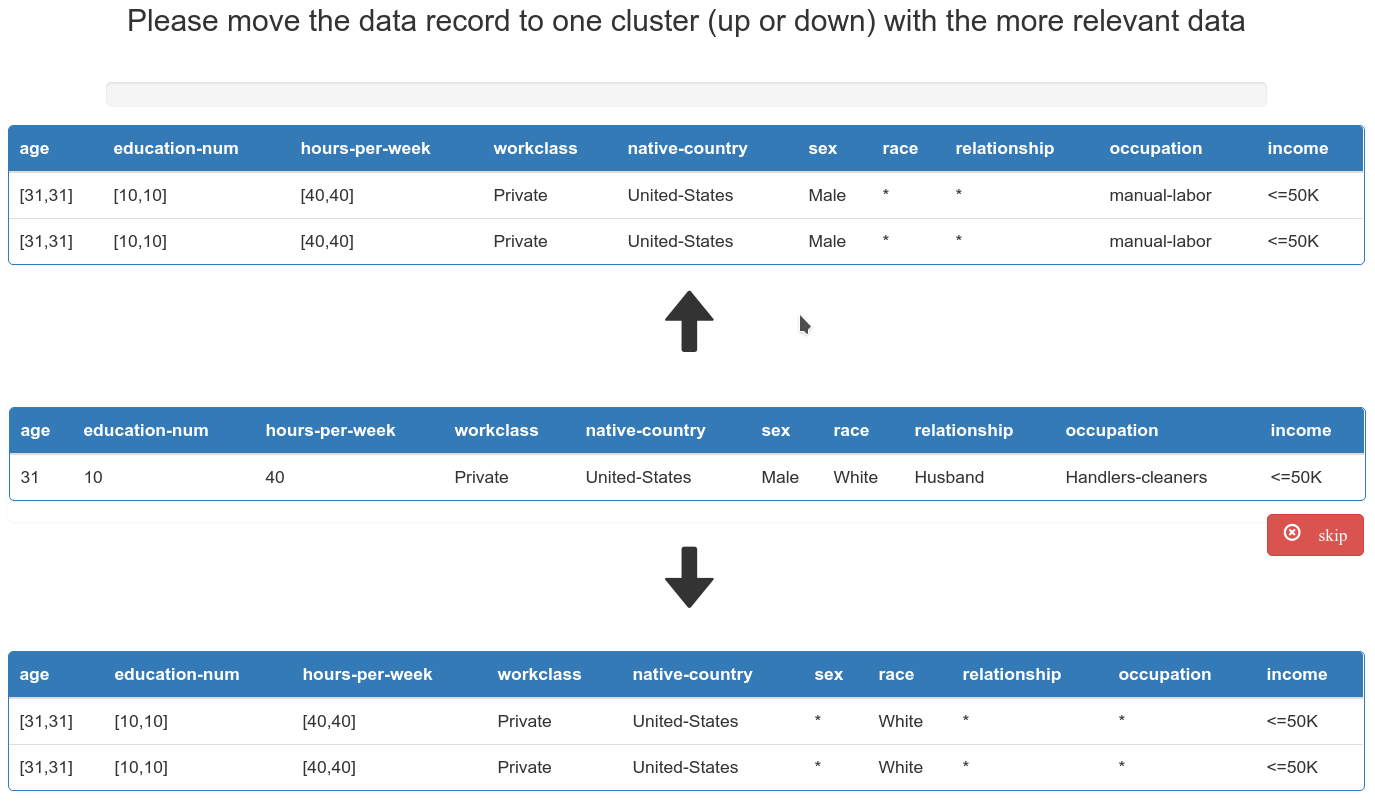
\includegraphics[width=1.0\textwidth]{figures/iml_anon_screen1}
		
		\vspace{1.0cm}
		\hspace*{-0.8cm}
		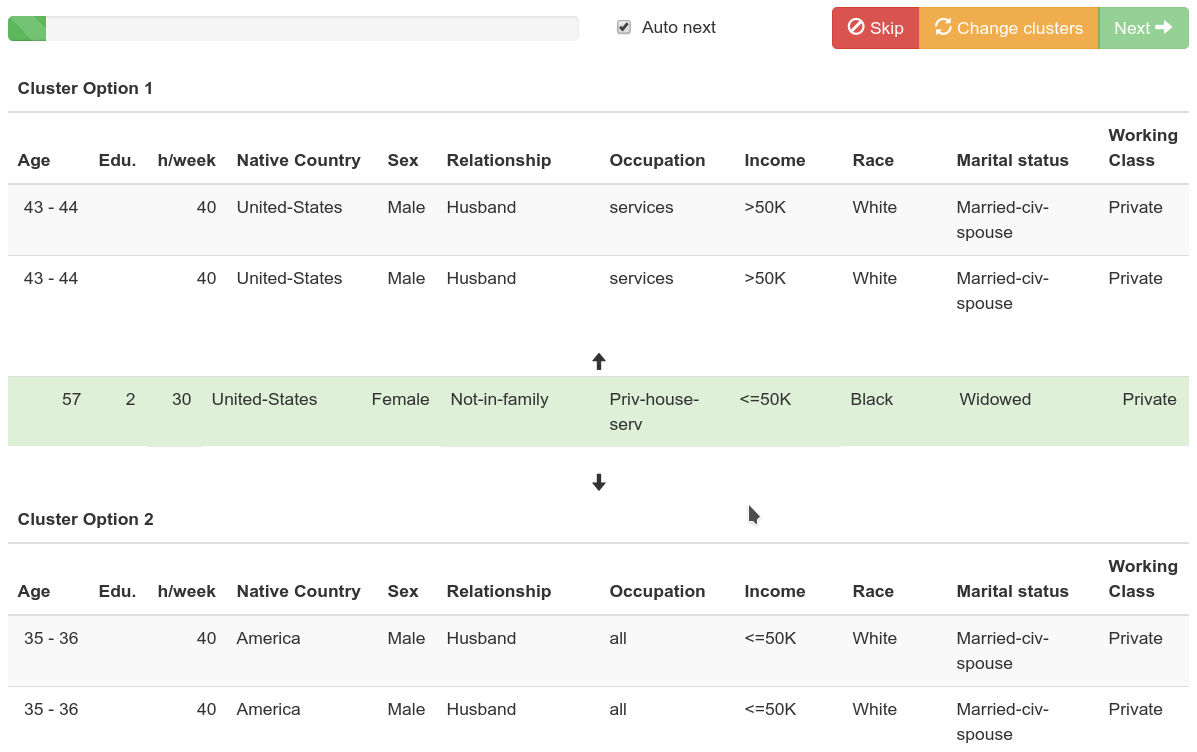
\includegraphics[width=1.0\textwidth]{figures/iml_anon_screen2}
		\caption{Two different implementations of the iML interface design.}
		\label{fig:iml_UI}
	\end{center}
\end{figure}


\subsection{Data} 
\label{ssect:data}

We chose the adults dataset from the UCI Machine Learning repository which was generated from US census data from 1994 and contains approximately 50k entries in it's original; after initial preprocessing we chose the first 500 complete data rows as our iML experimental data to be presented to users via a Web Browser UI. After obtaining bias / iml weights from the experiment, we chose the first 3k entries of the original data as the basis for producing 775 new, anonymized data sets. Although 3k rows might seem overly frugal on our part, we have asserted via random deletion of original data points that classifier performance remains stable for as little as 1.5k randomly selected rows. Of the original attributes (data columns) provided 4 were deleted: 'capital-gain' \& 'capital-loss' (both were too skewed to be useful for humans), 'fnlwgt' (a mere weighting factor) as well as 'education' which is also represented by a column containing its numerical mapping ('education\_num').


\subsection{Anonymization Algorithm}
\label{ssect:algorithm}

In order to conduct our experiments, it was necessary to choose an algorithm which would enable us to easily hook into its internal logic - we therefore chose a greedy clustering algorithm called \textit{SaNGreeA} (Social network greedy clustering) which was introduced by \cite{campan2009data} and implemented it in JavaScript. This enabled us to execute it within a browser environment during our iML experiments as well as server-side for batch-execution of all derived datasets afterwards.

Besides its capacity to anonymize graph structures (which we did not utilize during this work), it is a relatively simple algorithm considering \textit{General information loss} - or GIL - during anonymization. This GIL can be interpreted by the sum of information loss occurring during generalization of continuous (range) as well as hierarchical attributes:

\begin{equation*}
\begin{split}
\text{GIL}(cl) = \abs{cl} \cdot (\sum_{j=1}^{s} \frac{size(gen(cl)[N_j])}{size(min_{x \epsilon N} (X[N_j]), max_{x \epsilon N} (X[N_j]))} \\
+ \sum_{j=1}^{t} \frac{height(\Lambda(gen(cl)[C_j]))}{height(H_{C_j})})
\end{split}
\end{equation*}


where:\\
- $\abs{cl}$ denotes the cluster cl's cardinality; \\
- $size([i1,i2])$ is the size of the interval $[i1,i2]$, i.e., $(i2-i1)$; \\
- $\Lambda(w), w \epsilon H_{C_j}$ is the sub-hierarchy of $H_{C_j}$ rooted in $w$; \\
- $height(H_{C_j})$ denotes the height of the tree hierarchy $H_{C_j}$; \\


The following formulas then give the total / normalized GIL, respectively:
\begin{equation*}
\text{GIL}(G,S) = \sum_{j=1}^{v} \text{GIL}(cl_j) \quad \textrm{and} \quad
\text{NGIL}(G,S) = \frac{\text{GIL}(G,S)}{n \cdot (s+t)}
\end{equation*}

The algorithm starts by picking a (random or pre-defined) data row as its first cluster, then iteratively picking best candidates for merging by minimizing GIL until the cluster reaches size $k$, at which point a new data point is chosen as the initiator for the next cluster; this process continues until all data points are merged into clusters, satisfying the $k$-anonymity criterion for the given dataset.


\subsection{Processing pipeline for obtaining results}
\label{ssect:process}

Once our iML experiments had yielded enough weight vectors, we had to generate a whole new set of anonymized datasets on which we subsequently applied 4 classifiers on each of the 3 target attributes (columns) described; therefore we designed the following processing pipeline:


\begin{enumerate}
	\item Taking the first 5k rows of the original, preprocessed dataset as input and applying k-anonymization with a k-factor range of [5, 10, 20, 50, 100, 200] and 129 different weight vectors (equal, bias, iml) from our experiments on it, we produced 774 anonymized datasets (775 including the original).
	\item We then executed 4 different classifiers on all of the datasets and computed precision, recall as well as F1 score. The four classifiers used were \textit{linear SVC} (as a representative of Support Vector Machines), \textit{logistic regression} (gradient descent), \textit{gradient boosting} (ensemble, boosting) as well as \textit{random forest} (ensemble, bagging). While reading the datasets pertaining to the classification target of \textit{education}, the 14 different education levels present within the adult dataset were grouped into 4 categories 'pre-high-school', 'high school', '$<=$bachelors' and 'advanced studies'.
	\item For each combination of classification target (\textit{income}, \textit{marital status}, \textit{education}) and weight category (\textit{equal}, \textit{bias}, \textit{iml}) we averaged the respective results. Results were plotted per target, as this allows better comparison between different classifiers. The leftmost point in all plots designates the original, un-anonymized dataset.
\end{enumerate}


% ==================================
%		RESULTS & DISCUSSION
% ==================================
\section{Results \& Discussion}
\label{sect:results}

As per the results in our initial PaML paper \cite{malle2016right} as well as hitherto unpublished subsequent studies we generally expected $1/x$ shaped curves for classifier performance as factors of $k$ are increasing. These expectations held to only a small degree; moreover for targets \textit{education} as well as \textit{income} there was no clear winner amongst the weight categories, with some achieving better or worse depending on a specific factor of $k$.

We got the smoothest results for the \textit{marital status} target, with human bias winning consistently over equal weights as well as human interaction Figure~\ref{fig:results_marital}. We interpret this as stemming from the fact that there is a significant correlation between the attributes 'marital-status' and 'relationship' in the dataset, which led users to consciously overvalue the latter when prompted for their bias. It is not completely clear why the iML results were not able to keep up in this case, but since this seems to be a general phenomenon throughout our results, we will discuss this in a later paragraph.

\begin{figure}[!h]
	\begin{center}
		\hspace*{-0.8cm}
		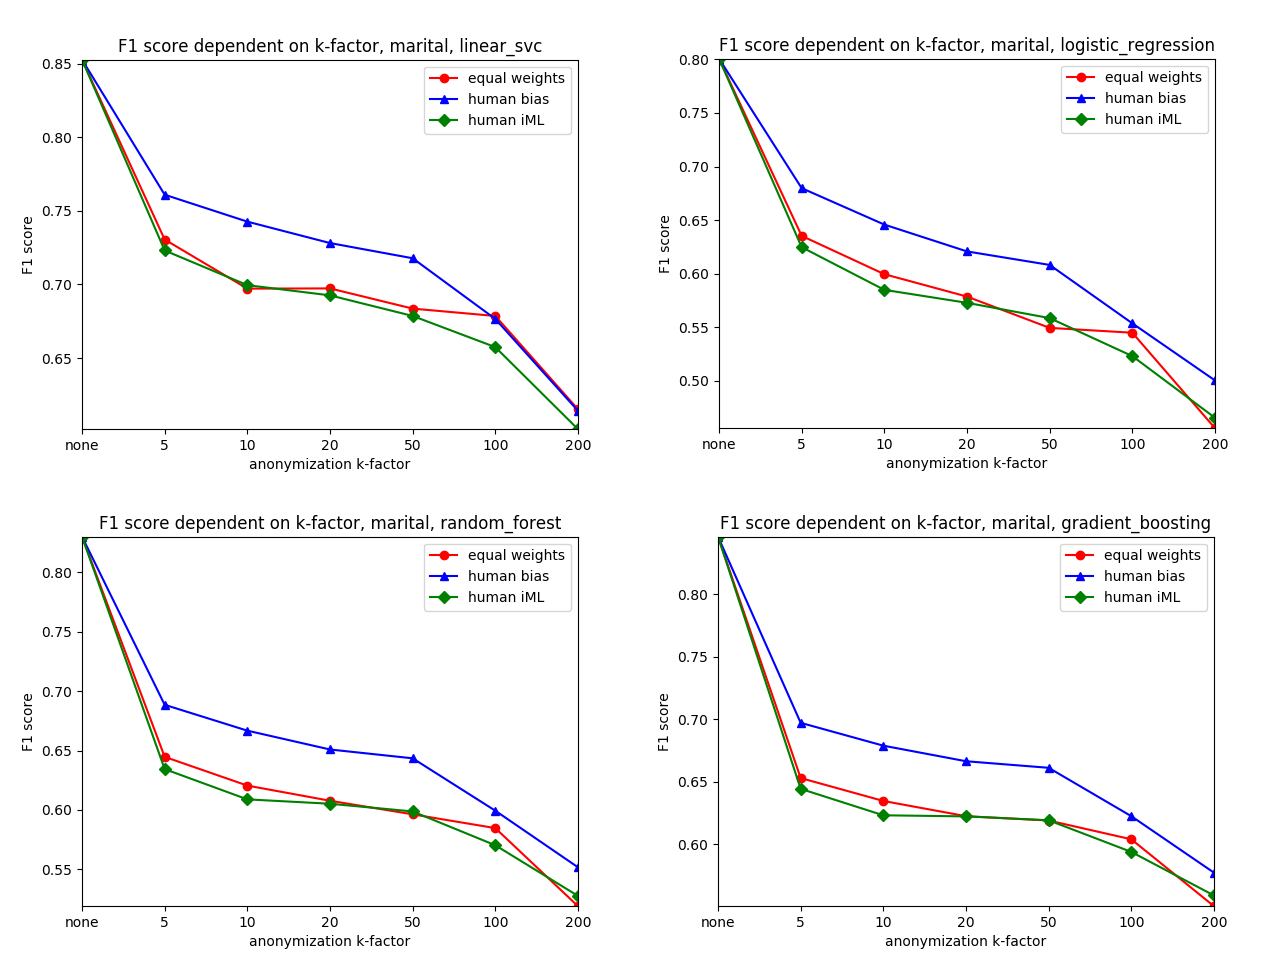
\includegraphics[width=1.1\textwidth]{figures/marital_status.png}
		\caption{Results on target \textit{marital status} - human bias wins consistently over both equal weights and human interaction with the algorithm.}
		\label{fig:results_marital}
	\end{center}
\end{figure}


On classification target \textit{education}, bias still mostly outperforms iML-obtained attribute weights, with equal weights slightly winning out at very high factors of $k$. Although we assume that apparently important clues towards education might be misleading (like income or working hours), this cannot explain the difference between bias- and iML-based results. It has to be noted however, that results on this target are distinctly inferior to those of the other scenarios which might diminish the gap's significance.

\begin{figure}[!h]
	\begin{center}
		\hspace*{-0.8cm}
		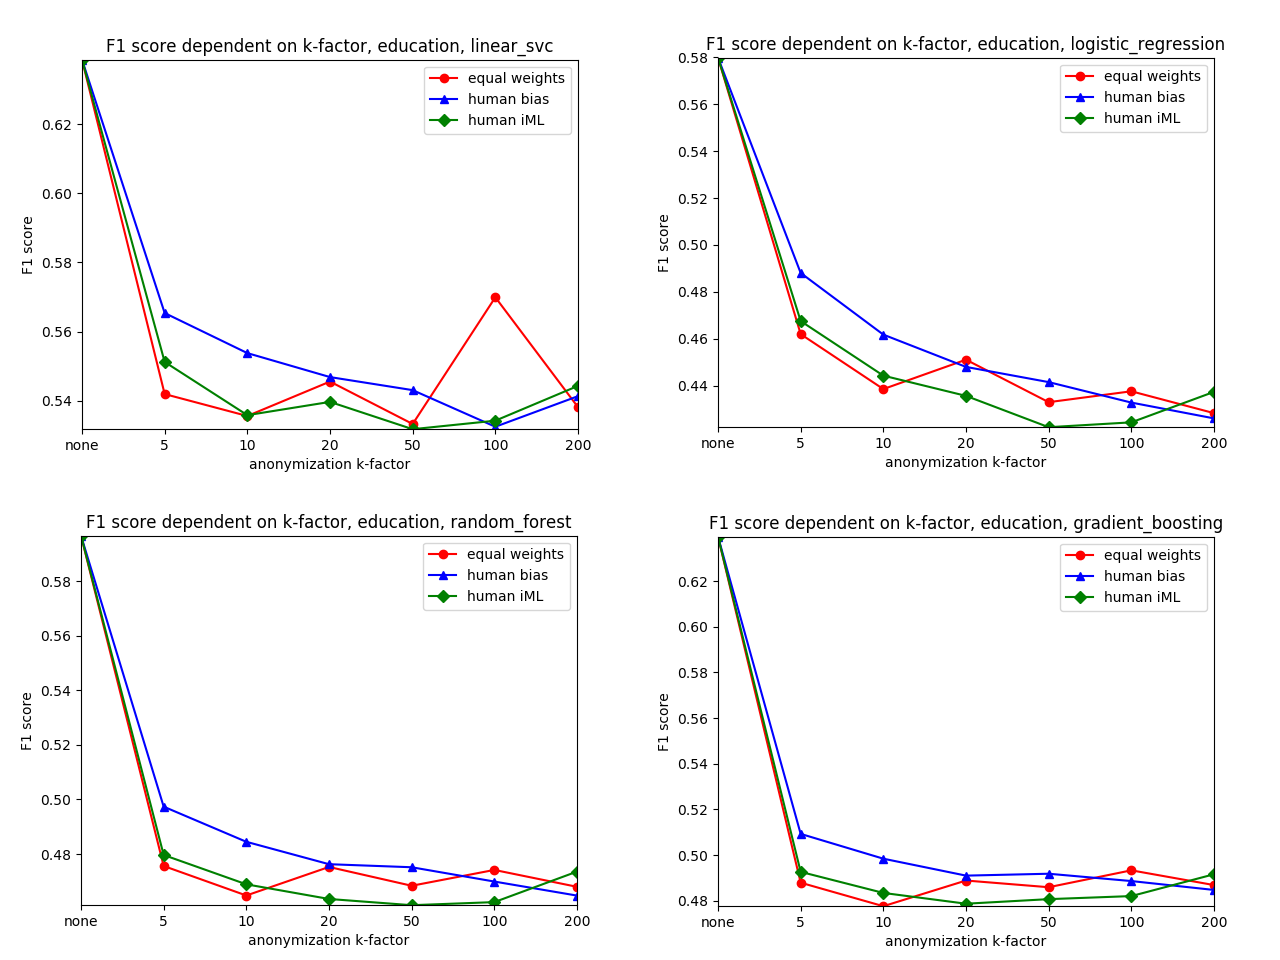
\includegraphics[width=1.1\textwidth]{figures/education_num.png}
		\caption{Results on target \textit{education} - we still see human bias performing slightly better than equal weights / iML in most cases of $k$, but not as consequently as above.}
		\label{fig:results_education}
	\end{center}
\end{figure}


Only on target \textit{income} did we observe a partly reversed order between human bias and iML - however at the cost of both being usually inferior to a simple setting with equal attribute weights. This is especially surprising because \textit{income} was the only binary classification task in our experiments, which should have given humans a slight advantage over the algorithm. On the other hand, human bias seems most susceptible to falling prey to certain stereotypes in the area of money (w.r.t. gender, race, marital status...), which would explain the reversal of results.

\begin{figure}[!h]
	\begin{center}
		\hspace*{-0.8cm}
		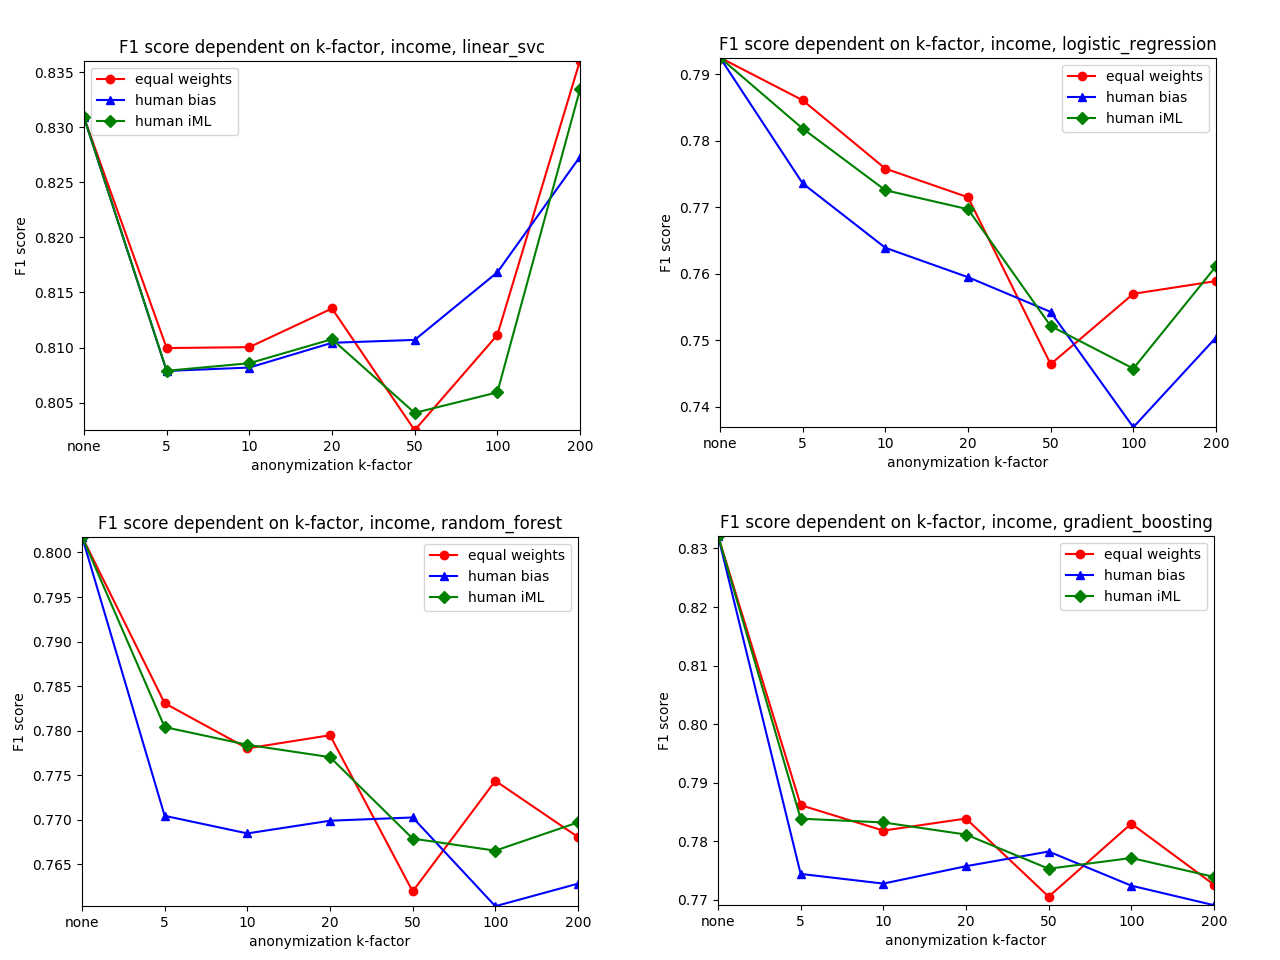
\includegraphics[width=1.1\textwidth]{figures/income.png}
		\caption{Results on target \textit{income} - only in this scenario do we see iML-based results generally outperforming bias (except linear SVC), nevertheless incapable of outperforming the rigidly equal setting.}
		\label{fig:results_income}
	\end{center}
\end{figure}

As for the failure of iML to significantly outperform both the equal weight setting and especially human bias, we conjecture that our experimental setup has produced those effects: Since we wanted our users to conduct their experiment in real-time but needed a simple implementation of an anonymization algorithm to enable this interaction (which resulted in an $O(n^2)$ algorithmic runtime), we had to limit ourselves to just a tiny subset of data (500 rows, merely 1\% of the original dataset). This choice apparently resulted in generalizations proceeding far too quickly, reaching suppression ('all') levels prematurely, thereby denying our users sensible clustering choices. On the other hand, the effect could also stem from users not really trying to contribute to the experiments in a meaningful way; this effect could only be mitigated by selecting more serious users or choosing some less serious (more social?) application domain.

Overall, we were also surprised that a seemingly absurd $k$-factor of 200 would still yield comparably good results (and in some cases even improve performance..).

% ==================================
%		PROBLEMS & CHALLENGES
% ==================================
\section{Open problems \& future challenges}
\label{sect:op_fc}

As iML for anonymization is still a fledgling sub-area in the larger fields of privacy as well as Machine Learning, there are certainly innumerable possibilities for even basic progress \& development. The following list is only a tiny subset of possible research venues we deem suitable for our own future work:

\begin{itemize}
	\item \textbf{Explain the unexpected behavior} of linear SVC on the \textit{income} target at high levels of $k$; probably by performing comparison studies on synthetically generated datasets.
	\item \textbf{Faster algorithm.} Repeat the experiments with a faster algorithmic implementation so that we can use thousands of data points even in real time within a Browser: this would lead to more relaxed generalizations, allowing the user to make better interactive choices, thus presumably improving results by quite some margin.
	\item \textbf{Expert domain, domain experts.} Choosing an expert domain like cancer studies in combination with proper experts like medical professionals, we would expect both human bias as well as iML results to significantly outperform a pre-defined weight vector.
	\item \textbf{Different setting.} On the other hand, a more 'gamified' setting such as recommendations within a social network could motivate amateur users to get more immersed into the experiment, yielding better results even for mundane application tasks.
	\item \textbf{Different data formats.} As Artificial Intelligence is slowly reaching maturity, it is now also applied to non-structured data like audio, images or even video. Since images are clearly relevant for medical research, and humans extremely efficient at processing them, studying interactive ML on visual data promises great scientific revenue. 
\end{itemize}


% ==================================
%			CONCLUSION
% ==================================
\section{Conclusion}
\label{sect:conclusion}

Based on the emerging necessity of Privacy aware data processing, in this work we presented a fundamental approach of bringing human knowledge to bear on the task of anonymization via interactive Machine Learning. We devised an experiment involving clustering of data points with respect to human preference for attribute preservation and tested the resulting parameters on classification of anonymized people data into classes of \textit{marital status}, \textit{education} and \textit{income}. Our preliminary results show that human bias can definitely contribute to even mundane application areas, whereas more complex or convoluted tasks may require trained professionals or better data preparation (dimensionality reduction etc.). We also described our insights regarding technical details for iML experiments and closed by outlining promising future research venues.


\bibliographystyle{plain}
\bibliography{references}

\end{document}

